% Compilar na pasta deste arquivo com LuaLaTeX.
% Foto e fontes locais estão em assets/; mantenha essa pasta junto ao .tex.
\documentclass[11pt,a4paper]{article}
\usepackage[margin=16mm]{geometry}
\usepackage{fontspec}
\usepackage[brazil]{babel}
\usepackage{graphicx,tikz,enumitem}
\usepackage[hidelinks]{hyperref}
\setmainfont{SourceSans3}[Path=assets/fonts/,Extension=.otf,
  UprightFont=*-Regular,BoldFont=*-Bold,ItalicFont=*-It]
\newfontfamily\solidicons{fa-solid-900.ttf}[Path=assets/fonts/]
\newfontfamily\brandicons{fa-brands-400.ttf}[Path=assets/fonts/]
\hypersetup{pdftitle={Kleber Daniel Mattos Viana Resume},pdfauthor={Kleber Daniel Mattos Viana}}
\pagestyle{empty}
\setlength{\parindent}{0pt}
\setlength{\parskip}{0pt}
\setlist[itemize]{leftmargin=10pt,labelsep=4pt,itemsep=0pt,parsep=0pt,topsep=0pt,label=\textbullet}
\newcommand{\cvsection}[1]{\par\vspace{15pt}{\fontsize{12}{15}\selectfont\bfseries #1\par}\vspace{2pt}\hrule height 1.2pt\vspace{7pt}}
\newcommand{\external}{\,\raisebox{.1ex}{\fontsize{6}{6}\selectfont\solidicons\symbol{"F35D}}}
\newcommand{\linked}[2]{\href{#1}{#2\external}}
\newcommand{\entry}[3]{\par\noindent\begin{minipage}[t]{.78\linewidth}#1\end{minipage}\hfill\begin{minipage}[t]{.20\linewidth}\raggedleft #2\if\relax\detokenize{#3}\relax\else\\#3\fi\end{minipage}\par}
\begin{document}
\fontsize{11}{14.3}\selectfont
\begin{center}
\begin{tikzpicture}
\clip (0,0) circle (13mm);
\node[inner sep=0pt] at (0,0) {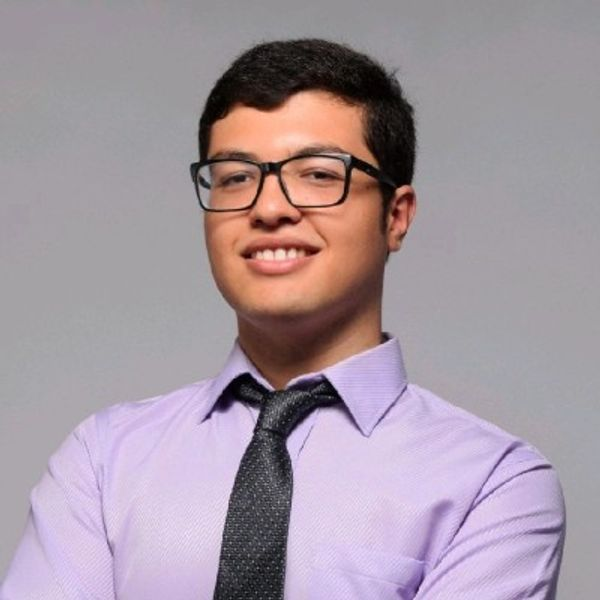
\includegraphics[width=26mm]{assets/foto.jpg}};
\end{tikzpicture}\par
\vspace{4pt}
{\fontsize{19}{23}\selectfont\bfseries Kleber Daniel Mattos Viana\par}
\vspace{4pt}
{\fontsize{12.5}{16}\selectfont Software Engineer | Python Backend | Automação de Estudos Elétricos\par}
\vspace{6pt}
\href{mailto:danielcmc100@gmail.com}{{\solidicons\symbol{"F0E0}}\enspace danielcmc100@gmail.com}\quad
\href{tel:+5521975176594}{{\solidicons\symbol{"F095}}\enspace +55 21 97517-6594}\quad
\href{https://github.com/Danielcmc100}{{\brandicons\symbol{"F09B}}\enspace github.com/Danielcmc100}\par
\vspace{6pt}
\href{https://www.linkedin.com/in/kleber-daniel-mattos-viana/}{{\brandicons\symbol{"F08C}}\enspace linkedin.com/in/kleber-daniel-mattos-viana}
\end{center}

\cvsection{Perfil}
Desenvolvedor de software com atuação na automação de estudos elétricos de alta tensão na PSTG-Tech. Experiência com Python, FastAPI e processamento de dados científicos, integrando ferramentas de engenharia ao Grid Singularity. Atuação na preparação de modelos, geração de cenários de simulação e elaboração automatizada de relatórios técnicos.

\cvsection{Experiência}
\entry{\textbf{Software Engineer}, \linked{https://www.linkedin.com/company/pstgtech/}{\textit{PSTG-Tech}}}{05/2024 -- Atual}{Teresópolis}
\vspace{4pt}
\begin{itemize}
\item Contribuí para a automação integrada de estudos elétricos no Grid Singularity, reduzindo o prazo de realização de pacotes de estudos de meses para dias, conforme estimativa operacional da equipe.
\item Automação da preparação de casos a partir de dados ANAREDE/ANAFAS e geração de cenários ATP para energização, religamento e rejeição de carga, com seleção de condições operativas N-1.
\item Desenvolvimento de conversor programático XML\textrightarrow ATP, com tratamento da conectividade elétrica e validação comparativa com arquivos gerados pelo ATPDraw.
\item Implementação de leitor binário nativo de arquivos \texttt{.pl4} e processamento de arquivos \texttt{.lis}, incluindo classificação de resultados, seleção de piores casos e geração de gráficos, tabelas e relatórios técnicos.
\item Desenvolvimento de APIs FastAPI para modelagem de componentes e orquestração de estudos, com tarefas assíncronas reexecutáveis, persistência de entradas e acompanhamento de progresso.
\item Integração com infraestrutura de simulação e ferramentas executadas via Wine em Linux, com uso de Docker, CI/CD e logs correlacionados por tarefa e estudo.
\end{itemize}
\vspace{9pt}
\entry{\textbf{Projeto de Iniciação Científica}, \linked{https://drive.google.com/file/d/1wcRFSVA4bPcsmzlGtsreWYLOCZH3ikjs/view?usp=drive_link}{\textit{UNIFESO}}\\Pesquisa em imagens médicas, aprendizado de máquina e conjuntos de dados.}{04/2024 -- 12/2025}{Teresópolis}

\cvsection{Habilidades}
\begin{minipage}[t]{.48\linewidth}\raggedright
\textbf{Desenvolvimento backend}\\
Python, FastAPI, APIs REST, programação assíncrona, Pydantic e SQLAlchemy/SQLModel
\par\vspace{12pt}
\textbf{Automação de estudos elétricos}\\
Integração ATP/ATPDraw e ANAREDE/ANAFAS, geração de cenários, conversão XML\textrightarrow ATP e geração de relatórios técnicos
\end{minipage}\hfill
\begin{minipage}[t]{.48\linewidth}\raggedright
\textbf{Dados e computação científica}\\
NumPy, Polars, Pandas, Matplotlib e processamento de arquivos de simulação
\par\vspace{12pt}
\textbf{Qualidade e infraestrutura}\\
pytest, Git, Linux, Docker, Wine e CI/CD
\end{minipage}

% Experiência e habilidades na primeira página; detalhes complementares na segunda.
\newpage
\cvsection{Projetos}
\entry{\linked{https://singularity.pstg.com.br/en/}{\textbf{Grid Singularity}}, \textit{Automação de estudos elétricos}}{2024 -- Atual}{}
Plataforma para preparação de modelos, geração de cenários ATP e pós-processamento de estudos de alta tensão. Abrange energização de linhas e transformadores, religamento monopolar e tripolar e rejeição de carga, além de relatórios de energização de bancos de capacitores.
\par\vspace{5pt}
\textbf{Tecnologias:} Python, FastAPI, NumPy, Polars, Pandas, SQLAlchemy, Docker e Linux.\\
\textbf{Integrações:} ANAREDE, ANAFAS, ATPDraw e ATP.
\par\vspace{10pt}
\linked{https://github.com/Danielcmc100/PDVPOOAV2}{\textbf{Ponto de venda}}\\
Sistema de ponto de venda desenvolvido com FastAPI.

\cvsection{Educação}
\entry{\textbf{Bacharelado}, \linked{https://www.unifeso.edu.br/cursos/graduacao/ciencia-da-computacao}{\textit{Ciência da Computação - Unifeso}}}{2023 -- 2026}{}

\cvsection{Cursos}
\entry{\textbf{CS50}, \textit{Harvard University}}{2024}{}
\begin{minipage}[t]{.76\linewidth}\raggedright
Fundamentos de ciência da computação, algoritmos, estruturas de dados e desenvolvimento de software.
\par\vspace{10pt}
\textbf{Desenvolvimento de Aplicações Backend}\\
Desenvolvimento de aplicações backend e APIs.
\end{minipage}

\cvsection{Línguas}
\textbf{Inglês}\\
Técnico
\end{document}
